\documentclass{beamer}
\usetheme{BauhausNeuralFEM} 
\usepackage{amssymb}

\usepackage{algpseudocode}

% --- Title info ---
\title[Discrete Form]{From FEM to Neural Operators: Scientific Machine Learning for Computational Mechanics\\[0.4cm]}
\subtitle{Discretizing the Weak Form}
\author{Dr-Ing Jorge Alberto L\'{o}pez Zerme\~{n}o}
\date{}

\graphicspath {{Figures/}}

\begin{document}

{
	\usebackgroundtemplate{
		\begin{tikzpicture}[remember picture,overlay]
			\node[opacity=0.25,inner sep=0pt] at (current page.center)
			{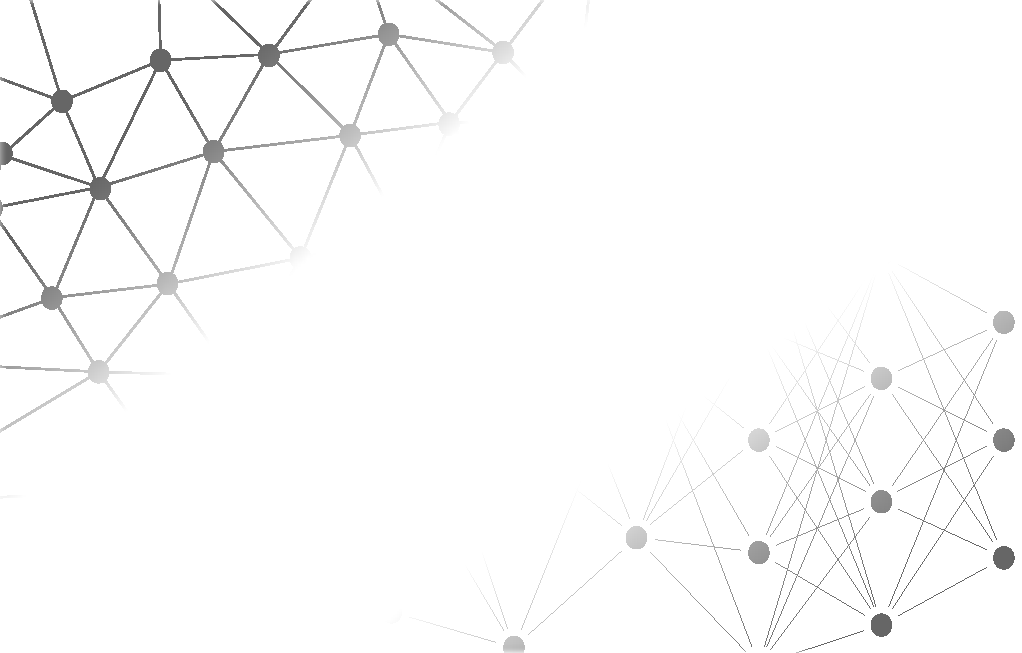
\includegraphics[width=\paperwidth,height=\paperheight]{Background.pdf}};
		\end{tikzpicture}
	}
	\begin{frame}[plain]
		\centering
		\begin{minipage}{0.21\textwidth}
			\centering
			
\includegraphics[width=\linewidth]{Bauhaus_Logo.png}
		\end{minipage}\hspace{105pt}
		\begin{minipage}{0.3\textwidth}
			\centering
			
\includegraphics[width=\linewidth]{JHU_Logo.png}
		\end{minipage}
		
		\titlepage
		\vspace{-35pt}
		Bauhaus Spring School 2026
		
	\end{frame}
}


\begin{frame}{Starting Point: The Weak Form}
	\begin{block}{Weak form of the Poisson equation}
		\textbf{1D:}
		\vspace{5pt}
		
		\footnotesize
		\begin{minipage}{0.5\textwidth}
			\begin{center}
				
\includegraphics[width=0.8\linewidth]{Figures/Dirichlet_Neumann_1D.pdf}
			\end{center}
		\end{minipage}\hfill
		\begin{minipage}{0.4\textwidth}
			\begin{equation*}
				\int_{0}^{L} u'(x)\,v'(x)\,dx = \int_{0}^{L} f(x)\,v(x)\,dx
			\end{equation*}
		\end{minipage}
	
		\vspace{15pt}
		\normalsize\textbf{2D:}
		\vspace{5pt}
		
		\footnotesize
		\begin{minipage}{0.5\textwidth}
			\begin{center}
				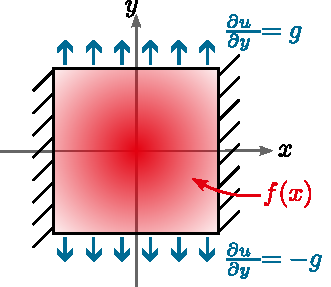
\includegraphics[width=0.8\linewidth]{Figures/Poisson_2D.pdf}
			\end{center}
		\end{minipage}\hfill
		\begin{minipage}{0.4\textwidth}
			\begin{equation*}
			\int_{\Omega} \nabla u \cdot \nabla v \, d\Omega = \int_{\Omega} f\,v\, d\Omega
			\end{equation*}
		\end{minipage}
	\end{block}
\end{frame}


\begin{frame}{Discrete Spaces (1D)}
	\begin{minipage}{0.5\textwidth}
		\begin{center}
			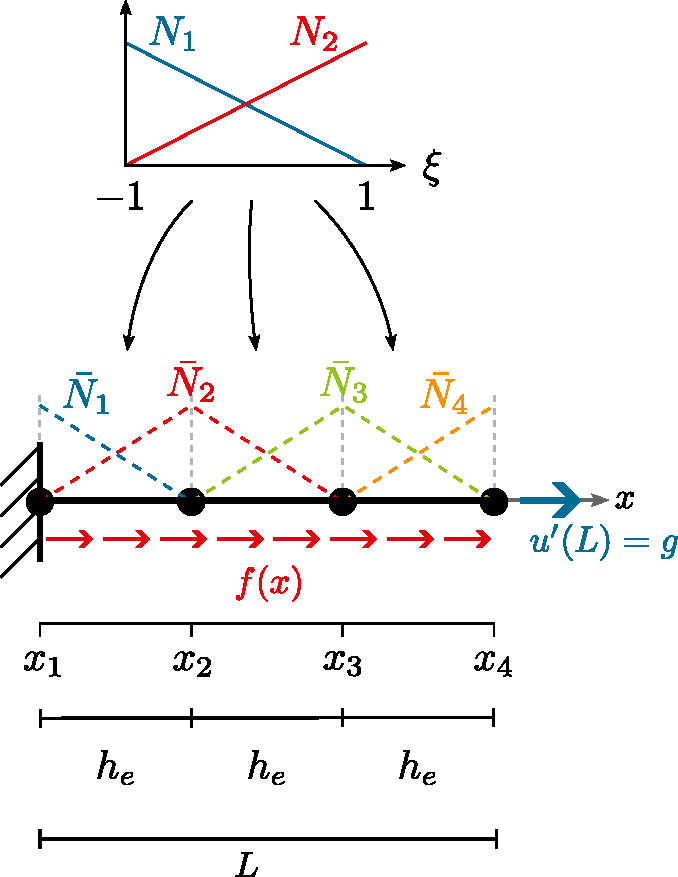
\includegraphics[width=\linewidth]{Figures/Global_Discretization.pdf}
		\end{center}
	\end{minipage}\hfill
	\begin{minipage}{0.47\textwidth}
		\normalsize
		\textbf{Global discretization:}
		\footnotesize
		\[
		u(x)&=\sum_{i=1}^{n} \bar{N}_i(x)\,u_i,\]
		\[
		v(x)&=\sum_{i=1}^{n} \bar{N}_i(x)\,v_i.
		\]
		
		\begin{itemize}
			\item $\bar{N}_i$ are assembled from shape functions on each element that share node \textit{i}.
			\item Local support.
		\end{itemize}
	
		\normalsize
		\textbf{Element level:}
		\footnotesize
		\[
		u_e(x)&=\sum_{i=1}^{n} N_i(x)\,u^e_i,\]
		\[
		v_e(x)&=\sum_{i=1}^{n} N_i(x)\,v^e_i.
		\]
	\end{minipage}
\end{frame}


\begin{frame}{From Weak Form to Discrete (Matrix) Form in 1D}
	\footnotesize
	\begin{minipage}{0.5\textwidth}
		\normalsize
		\textbf{Weak form:}
		\footnotesize
		\begin{equation*}
		\int_{he} u'(x)\,v'(x)\,dx = \int_{he} f(x)\,v(x)\,dx
		\end{equation*}
		
		\normalsize
		\textbf{Discretizing the gradients:}
		\footnotesize
		 \[
		u'_e(x)&=\sum_{i=1}^{n} N'_i(x)\,u^e_i,\quad
		v'_e(x)&=\sum_{i=1}^{n} N'_i(x)\,v^e_i.
		\]
	\end{minipage}\hfill
	\begin{minipage}{0.4\textwidth}
		\begin{center}
			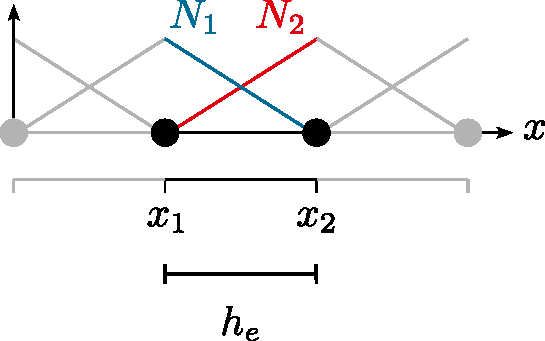
\includegraphics[width=\linewidth]{Figures/FEM_1D_Local_Basis.pdf}
		\end{center}
	\end{minipage}
	
  
  
  
 \vspace{15pt}
   
  \[
  \sum_{i=1}^{n}\sum_{j=1}^{n}\int_{he} N'_i(x)\,u^e_i N'_j(x)\,v^e_j\,dx = \sum_{j=1}^{n}\int_{he} f(x)\,N'_i(x)\,v^e_i\,dx
  \]
  \vspace{0.3em}
  \[
    K_{ij}= \int_{0}^{L} N_i'(x)\,N_j'(x)\,dx, \qquad
    f_i = \int_{0}^{L} f(x)\,N_i(x)\,dx
  \]
  \vspace{0.25em}
  \[
    \Rightarrow\quad \mathbf{K}\,\mathbf{u}=\mathbf{f}.
  \]

\end{frame}

% ------------------------- Slide 5 -------------------------
\begin{frame}{From Weak Form to Discrete (Matrix) Form in 2D}
  \begin{minipage}{0.38\textwidth}
  	\footnotesize
  	\begin{equation*}
  	\nabla N_a = \mathbf{J}^{-1}\,\nabla_{\!\xi} N_a,\quad \mathbf{J}=\begin{bmatrix}
  	\dfrac{\partial x}{\partial \xi} & \dfrac{\partial y}{\partial \xi}\\[0.5em]
  	\dfrac{\partial x}{\partial \eta} & \dfrac{\partial y}{\partial \eta}
  	\end{bmatrix}
  	\end{equation*}
  \end{minipage}\hfill
  \begin{minipage}{0.53\textwidth}
  	\begin{center}
  		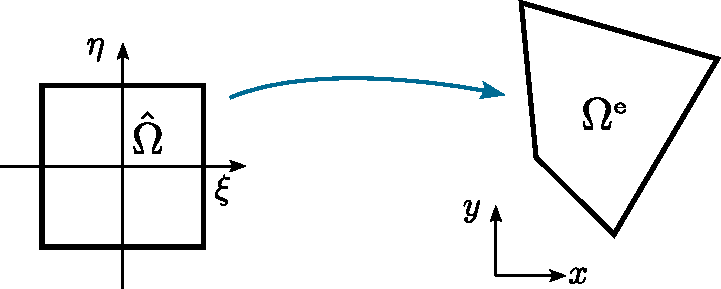
\includegraphics[width=\linewidth]{Figures/Iso_Mapping.pdf}
  	\end{center}
  \end{minipage}
  
  
  \begin{equation*}
  	\int_{\Omega} \nabla u \cdot \nabla v \, d\Omega = \int_{\Omega} f\,v\, d\Omega
  \end{equation*}
  
  \begin{equation*}
  	\nabla u = \sum_{i=1}\nabla N_i u_i, \quad \nabla v = \sum_{i=1}\nabla N_i v_i
  \end{equation*}
  
  \begin{equation*}
  \sum_{i=1}\sum_{j=1}\int_{\Omega} \nabla N_i u_i \cdot \nabla N_j v_j \, d\Omega = \sum_{i=1}\int_{\Omega} f\,N_i v_i\, d\Omega
  \end{equation*}
  \vspace{0.3em}
  \[
    K_{ij}= \int_{\Omega} \nabla N_i \cdot \nabla N_j \, d\Omega, \qquad
    f_i = \int_{\Omega} f\,N_i \, d\Omega
  \]
  \vspace{0.4em}
  
\end{frame}



\begin{frame}{Element Loop Algorithm}
	\begin{minipage}{0.42\textwidth}
		\small\textbf{Gauss Integration:}
		\begin{center}
			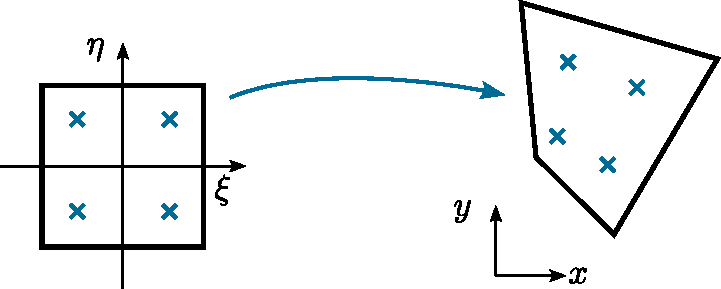
\includegraphics[width=\linewidth]{Figures/Mapping_in_Gauss.pdf}
		\end{center}
		
		\small\textbf{1D (per element):}
		\footnotesize
		\begin{align*}
			K^{(e)}_{ab} &\approx \sum_{q} w_q\,
			\frac{dN_b}{dx}\big|_{\xi_q}\,
			\frac{dN_a}{dx}\big|_{\xi_q}\,
			\big|J(\xi_q)\big|\\[3pt]
			f^{(e)}_{a} &\approx \sum_{q} w_q\, f(x_q)\, N_a(\xi_q)\,\big|J(\xi_q)\big|
		\end{align*}
		
		\vspace{-2pt}
		\small\textbf{2D (per element):}
		\footnotesize
		\begin{align*}
			K^{(e)}_{ab} &\approx \sum_{q} w_q\,
			\big(\nabla N_b \cdot \nabla N_a\big)\big|_{(\xi_q,\eta_q)}\,
			\big|\mathbf{J}(\xi_q,\eta_q)\big|\\[3pt]
			f^{(e)}_{a} &\approx \sum_{q} w_q\, f(\mathbf{x}_q)\, N_a(\xi_q,\eta_q)\,
			\big|\mathbf{J}(\xi_q,\eta_q)\big|
		\end{align*}
	\end{minipage}\hfill
	\begin{minipage}{0.44\textwidth}
		\begin{block}{\small Pseudocode: $\mathbf{K}^{(e)}$ and $\mathbf{f}^{(e)}$}
			\tiny
			\begin{algorithmic}
				\State \textbf{Input:} Element node coordinates $\mathbf{x}_a$, \\ 
				Source term $f(x)$, \\
				Gauss points and weights $(\xi_{q}, \eta_{q}, w_q)$
				\State \textbf{Output:} Element stiffness matrix $\mathbf{K}^{(e)}$, \\
				Element load vector $\mathbf{f}^{(e)}$
				
				\State Initialize $\mathbf{K}^{(e)} \gets \mathbf{0}$, $\mathbf{f}^{(e)} \gets \mathbf{0}$
				
				\For{each Gauss point $q$ in the parent element}
				\State Evaluate \\
				$N_a(\xi_{q}, \eta_{q})$, $\nabla_{\xi} N_a(\xi_{q}, \eta_{q})$
				\State Compute Jacobian: \\
				$\mathbf{J} \gets \sum_a \mathbf{x}_a \otimes \nabla_{\xi} N_a$
				\State Compute $\big|\mathbf{J}\big|$, \quad and $\mathbf{J}^{-1}$
				\State Physical gradients: \\
				$\nabla N_a \gets \mathbf{J}^{-1} \nabla_{\xi} N_a$
				\State Physical point: \\
				$\mathbf{x}_q \gets \sum_a N_a(\xi_{q}, \eta_{q})\, \mathbf{x}_a$
				
				\For{each local node $a$}
				\For{each local node $b$}
				\State $K^{(e)}_{ab} \gets K^{(e)}_{ab} 
				+ w_q \, \big( \nabla N_b \cdot \nabla N_a \big) \, \big|\mathbf{J}\big|$
				\EndFor
				\State $f^{(e)}_a \gets f^{(e)}_a 
				+ w_q \, f(\mathbf{x}_q)\, N_a\, \big|\mathbf{J}\big|$
				\EndFor
				\EndFor
			\end{algorithmic}
		\end{block}
		
	\end{minipage}
\end{frame}


\end{document}
